\documentclass[a4paper, 12pt]{article}
\usepackage{listings} 
\usepackage{xcolor}
\usepackage{mdframed}
\usepackage{graphicx}
\usepackage{pgfplots}
\usepackage{float}
\usepackage{mathtools}
\usepackage[margin=1.00in]{geometry}
\DeclarePairedDelimiter\ceil{\lceil}{\rceil}
\DeclarePairedDelimiter\floor{\lfloor}{\rfloor}
\definecolor{code-gray}{gray}{0.93}

% Beginning of Document
\begin{document}

% Title
\title{ECE 443 - Project \#3}
\author{Collin Heist}
\date{\today}
\maketitle

% Table of Content and Listings
\pagenumbering{roman}
\tableofcontents
\lstlistoflistings
\newpage
\pagenumbering{arabic}

% Beginning of Report
\section{Implementation}

\subsection{Initialization}
The most obvious place to start was incorporating my old EEPROM, LCD and UART libraries. Luckily, they were functional back from the ECE 341 lab. I started with changing my hardware initialization function to include each library's initialization function, shown in \textbf{Listing~\ref{lst:hardware-init}}. \textit{Note, no code listings show any TraceAlyzer code to avoid clutter.}

	\begin{mdframed}[backgroundcolor=code-gray, roundcorner=10pt,
								innerleftmargin=5, innertopmargin=5, innerbottommargin=5]	
	\begin{lstlisting}[language=C, caption=Hardware Initialization, tabsize=2, label={lst:hardware-init}]
	static void init_hardware() {
		chipKIT_PRO_MX7_Setup();
		initialize_LCD();
		init_eeprom();
		initialize_uart1(19200, ODD_PARITY);	

		PORTSetPinsDigitalOut(IOPORT_B, SM_LEDS);
		LATBCLR = SM_LEDS;
	
		PORTSetPinsDigitalIn(IOPORT_G, BTN1);
	
		mCNOpen(CN_ON, CN8_ENABLE, 0);
		mCNSetIntPriority(1);
		mCNSetIntSubPriority(0);
		unsigned int x = PORTReadBits(IOPORT_G, BTN1);
		mCNClearIntFlag();
		mCNIntEnable(1);

		ConfigIntUART1(UART_ERR_INT_DIS | UART_RX_INT_EN |
			UART_INT_PR2 | UART_INT_SUB_PR0 | UART_TX_INT_DIS);

		INTEnableSystemMultiVectoredInt();
	}
	\end{lstlisting}
	\end{mdframed}
	
Of course, I also needed to declare \textbf{BTN1} as an input, and enable the change notice interrupt for that button. Similarly, I also configured the UART peripheral to trigger an interrupt on \textbf{RX} (or receive). Both of these interrupts required corresponding assembly files that allowed them to more appropriately work with the \textbf{FreeRTOS} task structure. Those files are \textbf{cn\_isr\_wrapper.S} and \textbf{uartRX\_isr\_wrapper.S}.
 
I chose a priority level of one for my change notice, and two for the UART because the user can theoretically enter characters in very rapid succession, but each button press requires at least 20 milliseconds to debounce. In addition to this, the responsiveness of a button press is largely dictated by the time it takes to read from the EEPROM, display to the LCD, and the project-stated one second delay between clearing the screen and writing a message -- all of which are orders of magnitude greater than the delay created by having the UART interrupt trigger.

\subsection{Program Design}
After the obvious project requirements were taken care of, I started designing the actual functionality of the program. I decided to utilize two semaphores, and two queues. Each wrapper ISR requires a semaphore in order to return to the desired wrapper task, so that much was obviously needed. And I used one queue to handle the 'stream' of addresses where the user-entered messages are stored in the EEPROM, and the second queue contains a list of pending retrieval requests. This pending retrieval queue has meaningless data, and I could have instead used a counting semaphore -- but this is functionally equivalent, and allows for additional data to be transmitted in the future (if necessary).

\subsection{Message Input \& EEPROM Writing}
The easiest component to implement was the UART handler. This required its own assembly wrapper file, and is triggered every time a character is entered on the UART interface (over Putty). Below, in \textbf{Listing~\ref{lst:uart-isr}}.

	\begin{mdframed}[backgroundcolor=code-gray, roundcorner=10pt,
								innerleftmargin=5, innertopmargin=5, innerbottommargin=5]	
	\begin{lstlisting}[language=C, caption=UART ISR Handler, tabsize=2, label={lst:uart-isr}]
	void isr_uart_RX_handler(void) {
		portBASE_TYPE move_to_higher_priority = pdFALSE;

		if (getStrU1(uart_input, sizeof(uart_input))) {
			putcU1('\n');
			xSemaphoreGiveFromISR(write_to_eeprom,
				&move_to_higher_priority);
			
			mPORTBClearBits(LEDA);
		}	

		mU1RXClearIntFlag();
	
		portEND_SWITCHING_ISR(move_to_higher_priority);
	}
	\end{lstlisting}
	\end{mdframed}
	
This interrupt is called from the assembly wrapper, and using the \textbf{getStrU1()} function written into my \textbf{comm} library, the buffer \textbf{uart\_input} is filled with the incoming message. This function returns true when a terminating character is detected, at which point a newline is echoed (to better format the Putty window), and then the semaphore is given to initiate a \emph{write} to the EEPROM. After a semaphore is given, the interrupt flag is cleared, and then a switch is initiated to either the calling task or the newly unblocked EEPROM writing \emph{task} -- which is shown below in \textbf{Listing~\ref{lst:task-eeprom-write}}.

	\begin{mdframed}[backgroundcolor=code-gray, roundcorner=10pt,
								innerleftmargin=5, innertopmargin=5, innerbottommargin=5]	
	\begin{lstlisting}[language=C, caption=EEPROM Writing Task, tabsize=2, label={lst:task-eeprom-write}]
	static void task_write_EEPROM(void *task_params) {
		unsigned int i = 0;
		static unsigned int eeprom_write_addr = 0;
		portBASE_TYPE queue_status;
	
		xSemaphoreTake(write_to_eeprom, 0);
		for (;;) {
			xSemaphoreTake(write_to_eeprom, portMAX_DELAY);

			if (uxQueueMessagesWaiting(eeprom_addr_queue) ==
				MAX_NUM_MSGS) {}
			else {
				unsigned int write_error = NO_ERR;
			
				write_error = write_eeprom(EEPROM_SLAVE_ADDR,
					eeprom_write_addr, uart_input, UART_MAX_MSG_SIZE);
				if (write_error) {}
				else {
					queue_status = xQueueSendToBack(eeprom_addr_queue,
						&eeprom_write_addr, 0);

					eeprom_write_addr += UART_MAX_MSG_SIZE;
					eeprom_write_addr %= UART_MAX_MSG_SIZE * MAX_NUM_MSGS;
				}
			}

			for (i = 0; i < UART_MAX_MSG_SIZE; i++)
				uart_input[i] = 0;

			if (uxQueueMessagesWaiting(eeprom_addr_queue)
				!= MAX_NUM_MSGS)
				mPORTBSetBits(LEDA);
		}
	}
	\end{lstlisting}
	\end{mdframed}
	
As with typical task functions, this is implemented with an infinite for loop. The loop blocks forever -- until the \textbf{write\_to\_eeprom} semaphore is given from the UART ISR handler (see \textbf{Listing~\ref{lst:uart-isr}}). The reception of this semaphore indicates that a complete message has been written into the \textbf{uart\_input} character buffer, and is ready to be written to the EEPROM. After the write is finished, the starting address of that message is sent to the address queue, and then the global address variable is incremented and wrapped back around (to enforce the message count limitation).

\subsection{EEPROM Reading \& LCD Writing}
After parsing and writing the messages, button presses need to initiate a read from the EEPROM and display that message to the LCD. For starters, all presses of button one activate the change-notice interrupt, shown below.

	\begin{mdframed}[backgroundcolor=code-gray, roundcorner=10pt,
								innerleftmargin=5, innertopmargin=5, innerbottommargin=5]	
	\begin{lstlisting}[language=C, caption=Change Notice ISR Handler, tabsize=2, label={lst:isr-change-notice-handler}]
	void isr_change_notice_handler(void) {
		portBASE_TYPE move_to_higher_priority = pdFALSE;
	
		xSemaphoreGiveFromISR(cn_semaphore,
			&move_to_higher_priority);
	
		mCNClearIntFlag();
		mCNOpen(CN_OFF, (CN8_ENABLE), 0);
	
		portEND_SWITCHING_ISR(move_to_higher_priority);
	}
	\end{lstlisting}
	\end{mdframed}
	
Very simply, a button press gives the \textbf{cn\_semaphore}, which unblocks the code shown in \textbf{Listing~\ref{lst:task-change-notice-handler}}, and then clears the change notice interrupt flag. I did not include a button debounce inside this function because task execution needs to continue to occur during that debounce period. The handler \emph{task} that is unblocked by the semaphore given in the change notice ISR handler executes a vast majority of the change notice code.

	\begin{mdframed}[backgroundcolor=code-gray, roundcorner=10pt,
								innerleftmargin=5, innertopmargin=5, innerbottommargin=5]	
	\begin{lstlisting}[language=C, caption=Change Notice Handler Task, tabsize=2, label={lst:task-change-notice-handler}]
	static void task_change_notice_handler(void *task_params) {
		portBASE_TYPE queue_status;
		unsigned int dummy_val = 1;
		unsigned int current_btn1_status = 0;
	
		xSemaphoreTake(cn_semaphore, 0);
		for (;;) {
			xSemaphoreTake(cn_semaphore, portMAX_DELAY);
			current_btn1_status = PORTG & BTN1;
			
			vTaskDelay(MS_TO_TICKS(DEBOUNCE_TIME_MS));
		
			if (previous_BTN1_status == 0 && current_btn1_status)
				queue_status = xQueueSendToBack(eeprom_pending_queue,
					&dummy_val, 0);
		
			previous_BTN1_status = current_btn1_status;
		}
	}
	\end{lstlisting}
	\end{mdframed}
	
This task waits for the change notice ISR semaphore forever, and once received the status of button 1 is read, and then a debounce is performed for \textbf{DEBOUNCE\_TIME\_MS} (default 20, in the header) milliseconds. After this blocking is finished, the previous button status is compared with the current button status (in order to detect only button \emph{presses} and not releases) and then a dummy value is added to the pending request queue. This was addressed earlier, but a counting semaphore could have been used here, but I chose to use a queue here because it was easier, and allows for more exchanging of information in the future. For this implementation, the very presence of a value in the pending queue indicates that a message \emph{wants} to be read from the EEPROM.

After a value is added to the pending queue, the below reading task unblocks. This task is shown in \textbf{Listing~\ref{lst:task-read-eeprom}}.

	\begin{mdframed}[backgroundcolor=code-gray, roundcorner=10pt,
								innerleftmargin=5, innertopmargin=5, innerbottommargin=5]	
	\begin{lstlisting}[language=C, caption=EEPROM Reading Task, tabsize=2, label={lst:task-read-eeprom}]
	static void task_read_EEPROM(void* task_params) {
		portBASE_TYPE queue_status;
		unsigned int eeprom_read_addr, dummy_val, i, line_index;

		for (;;) {
			char eeprom_message[UART_MAX_MSG_SIZE+1] = {0};
			char lcd_message[LCD_CHAR_WIDTH+1] = {0};

			xQueueReceive(eeprom_pending_queue, &dummy_val,
				portMAX_DELAY);
			queue_status = xQueueReceive(eeprom_addr_queue,
				&eeprom_read_addr, 0);
			if (queue_status == pdTRUE) {
				unsigned int read_error = NO_ERR;
				read_error = read_eeprom(EEPROM_SLAVE_ADDR,
					eeprom_read_addr, eeprom_message, UART_MAX_MSG_SIZE);

				format_message_LCD(eeprom_message, UART_MAX_MSG_SIZE,
					LCD_CHAR_WIDTH);
			
				unsigned int num_lines = get_line_count(eeprom_message,
					UART_MAX_MSG_SIZE);
			
				reset_clear_LCD();
				vTaskDelay(MS_TO_TICKS(LCD_BLANK_PERIOD_MS));
				set_cursor_LCD(SECOND_LINE_START);
				get_row_string(eeprom_message, UART_MAX_MSG_SIZE, 0,
					lcd_message, LCD_CHAR_WIDTH + 1);
				put_string_LCD(lcd_message);
			
				for (line_index = 1; line_index < num_lines + 1;
					line_index++) {
					
					vTaskDelay(MS_TO_TICKS(LCD_ROLLING_DELAY_MS));
					reset_clear_LCD();
					set_cursor_LCD(FIRST_LINE_START);
					get_row_string(eeprom_message, UART_MAX_MSG_SIZE,
						line_index - 1, lcd_message, LCD_CHAR_WIDTH + 1);
					put_string_LCD(lcd_message);
					set_cursor_LCD(SECOND_LINE_START);
					get_row_string(eeprom_message, UART_MAX_MSG_SIZE,
						line_index, lcd_message, LCD_CHAR_WIDTH + 1);
					put_string_LCD(lcd_message);
				}
			
				vTaskDelay(MS_TO_TICKS(LCD_ROLLING_DELAY_MS));
				reset_clear_LCD();	
				set_cursor_LCD(FIRST_LINE_START);
				get_row_string(eeprom_message, UART_MAX_MSG_SIZE,
					num_lines, lcd_message, LCD_CHAR_WIDTH + 1);
				put_string_LCD(lcd_message);
				vTaskDelay(MS_TO_TICKS(LCD_ROLLING_DELAY_MS));
				reset_clear_LCD();
			}
		}
	}
	\end{lstlisting}
	\end{mdframed}

This task accomplishes quite a lot. To begin, two character arrays are used: there is \textbf{eeprom\_message} that stores the message read from the EEPROM, and \textbf{lcd\_message} that keeps the temporary string being written to the LCD. The task blocks forever until the pending queue has dummy values in it, which happens in the button press handling task. After this, a value from the address queue (\textbf{eeprom\_addr\_queue}) is attempted to be read from. This read does not block at all so that the task finishes even if no data is available in the EEPROM. Assuming data had been previously written into the address queue, a read from the EEPROM is initiated at that address, and the result is stored in \textbf{eeprom\_message}. I then call \textbf{format\_message\_LCD()}, which is a function I wrote that loops through all characters in a provided character array, and replaces spaces with newline characters (\textbf{'$\backslash n$'}) where necessary, in order to have at most \textbf{LCD\_CHAR\_WIDTH} (16 for our case) characters on each 'line' of the LCD. This function changes the EEPROM message itself.

With the message formatted, I could the number of how many lines are in the message (from my \textbf{get\_line\_count()} function). This is used to loop through the message line-by-line. The LCD is cleared and kept blank for the desired delay (1000 ms in the guidelines) -- during this time other task execution may occur -- and then the LCD writing operations begin. The general outline of this is to loop through each line of the EEPROM message, storing the temporary string inside \textbf{lcd\_message}, and place that message on the second or first line of the LCD, and after the proper delay this is repeated. Finally, the LCD is cleared and the function exits.
 
\section{Testing \& Verification}
In order to validate this program, I added a lot of TraceAlyzer outputs whenever various events occur, these can be found in the original code source on the repository. 

\subsection{Message Write}
The first test was a generic message write, which would be initiated by a return-terminated message over the UART connection. Below, in \textbf{Figure~\ref{fig:message-write}}, is the TraceAlyzer output of this event. The one millisecond heartbeat task is ignored, as are the system outputs (kernel ticks, etc.), in all TraceAlyzer outputs.

\begin{figure}[H]
\centering
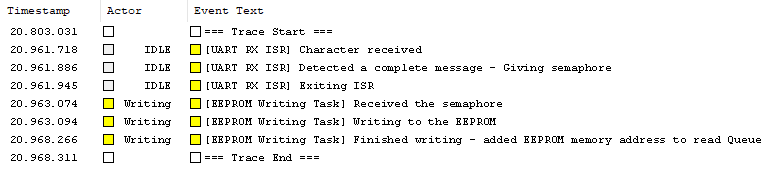
\includegraphics[width=\textwidth]{message-write.PNG}
\caption{TraceAlyzer event log of a complete message \textbf{write}, triggered by hitting return on the keyboard}
\label{fig:message-write}
\end{figure}

The sequence of events shown in this figure are as follows:

\begin{enumerate}
\item The return character is received over the UART interface - triggering the UART ISR.
\item \textbf{getStr()} returns true, signifying a complete message, resulting in the giving of the \textbf{write\_to\_eeprom} semaphore.
\item The UART ISR terminates and returned to the newly unblocked EEPROM writing task.
\item The message stored in \textbf{uart\_input} is written to the EEPROM.
\item The start address in EEPROM memory is added to the address queue.
\end{enumerate}

This sequence of events is exactly as I expect (and is desired) for a message reception.

\subsection{Message Read}
The next use-case I tested was a message retrieval initiated by a button press while a message was available to be read. Here's the TraceAlyzer output for this:

\begin{figure}[H]
\centering
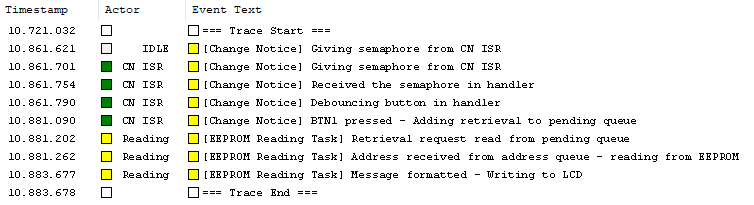
\includegraphics[width=\textwidth]{button-press.PNG}
\caption{TraceAlyzer event log of a message retrieval from the EEPROM, triggered by a press of \textbf{BTN1}}
\label{fig:button-press}
\end{figure}

Upon the button being pressed, the following happens:

\begin{enumerate}
\item The button press activates the change-notice ISR.
\item The handler ISR gives the \textbf{cn\_semaphore} and returns to the newly unblocked change notice handler task.
\item The handler task unblocks, and begins debouncing for 20 milliseconds.
\item After the debounce finishes, a button \emph{press} is detected, and a retrieval request is added to the pending queue.
\item The eeprom-reading task is now unblocked since the \textbf{eeprom\_pending\_queue} has a value in it -- starting a read from the EEPROM.
\item The message is read from the EEPROM, formatted, and written to the LCD.
\end{enumerate}

\subsection{Message Request With No Messages Available}
With these two 'typical' use-cases verified, I also checked more particular error-prone situations, such as a button press when \textbf{no} messages are available. This is shown in \textbf{Figure~\ref{fig:button-press-no-message}}.

\begin{figure}[H]
\centering
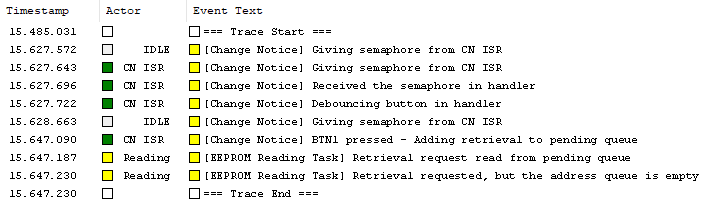
\includegraphics[width=\textwidth]{button-press-no-message.PNG}
\caption{TraceAlyzer event log of a message retrieval request with no available messages}
\label{fig:button-press-no-message}
\end{figure}

The events shown in this log are practically identical to those that occur in a normal message retrieval request, shown in \textbf{Figure~\ref{fig:button-press}}, except after the request queue unblocks, the non-blocking \textbf{xQueueReceive()} function call does not return \textbf{pdTRUE}, indicating a successful read from the queue. Because no addresses had been added to the queue, as no messages had been written to the EEPROM without already being read, the queue is empty and the system is unable to display anything on the LCD.

\subsection{User Enters More Than Five Messages}
Finally, I tested the situation where the user enters more than five messages at a time. I designed my program to work such that in this situation, nothing will happen to either the global address pointer, or the address queue. If TraceAlyzer is not being used, then technically the user will not know that this message is being ignored. The TraceAlyzer output is shown below:

\begin{figure}[H]
\centering
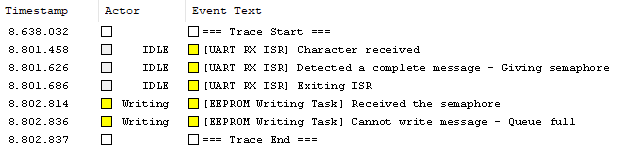
\includegraphics[width=\textwidth]{too-many-messages.PNG}
\caption{TraceAlyzer event log of the user entering more than five messages}
\label{fig:too-many-messages}
\end{figure}

\section{Design Overview}
I was able to avoid using global variables almost entirely. By using semaphore for initiating writing and reading from the EEPROM, and queues for transferring the sequences of address to read to, I alleviated the need for a lot of global arrays and variables.

If I wanted to avoid using \emph{any} global variables, I could have moved my global \textbf{uart\_message} character array to a queue that's the length of the maximum message. However, this takes up a lot of memory, and adds a significant amount of overhead with adding to and removing from queues, and would require me to manually take the input from the UART library, which adds to a character array, and add each character to a queue one-by-one. 

All in all, every component of my project works as desired. I also made many components of the design adjustable by changing the \textbf{\#define} statements inside \textbf{main.h}. You can change the following:

\begin{itemize}
\item \textbf{DEBOUNCE\_TIME\_MS} - How many milliseconds every press of \textbf{BTN1} is debounced
\item \textbf{UART\_MAX\_MSG\_SIZE} - The maximum allowed size of any one message entered over the UART
\item \textbf{MAX\_NUM\_MSGS} - The maximum number of messages stored in the EEPROM. If more messages are entered, they are simply ignored
\item \textbf{LCD\_CHAR\_WIDTH} - How wide the LCD is (in characters), can be changed to just change how the messages are displayed, does not need to match the actual width of the LCD
\item \textbf{LCD\_BLANK\_PERIOD\_MS} - How many milliseconds to blank the LCD before a message begins being displayed
\item \textbf{LCD\_ROLLING\_DELAY\_MS} - How many milliseconds to wait between each upward roll of the LCD
\end{itemize}

\end{document}